\chapter{Background and context}
\label{chap:background}
%\emph{This chapter contains all the information needed to put the thesis into context. It is common to use a revised version of your literature survey for this purpose. It is important to explicitly refer from your text to sources you have used, they will be listed in your bibliography.}

In this chapter we give more background information about the technology stack relevant to this thesis. Not all technologies are in use at the Lunatech's automotive client at the moment, nevertheless we include them to provide more information about similar technologies or new technologies that we could use in the future. We start with containers and container orchestration platforms which form the basics of running containerised workloads. Next we explore the different virtual networks technologies with \gls{cni}.

\section{Containers}
\label{sec:containers}
A Linux container is an isolated set of resources on a compute host. Containers work with namespacing: a container can only access resources in the same namespace and not any other namespaces. Meaning that a container can only see and modify its own processes and not other processes running in another container or on the host itself. Except for privileged containers which can use any resource and have access to every process on the host. 

Furthermore every container will get its own isolated network stack preventing privileged access to sockets and interfaces on other containers. One can create links and bridges to allow IP connectivity to and from a container.

Resource utilisation for containers is limited with \glspl{cgroup}. Giving each container a restricted set of resources, preventing the container to bring down the host by using too much RAM or CPU\cite{docker_security}.

\subsection{Docker}
\label{subsec:docker}
Docker is the standard in industry for running Linux containers. The Docker Engine is a container platform that makes it easy to run your container. You can run a container on your local developer machine and ship it, to run in a production environment.

It works with a Dockerfile to describe how to build your image. Every step will create a new file system layer and all layers together are your Docker image. You can reuse these layers between containers so that you can make a generic application container and add a layer on top for the specific application. This allows for reusability and will save storage and bandwidth when sharing images. The most popular way to share images is the Docker Hub, however one can also host a private Docker Registry to store and serve your own images.

\subsection{Kubernetes}
\label{subsec:kubernetes}
Kubernetes is an open-source container orchestration platform build from scratch, based on the ideas from the internal container engine used at Google. The basic scheduling unit in Kubernetes is a pod. A pod is collection of one or more containers that are co-located together on a host and share an unique IP address preventing port conflicts in the cluster. Pods allow you to run tightly coupled applications together.

Kubernetes consists of different loosely coupled components as can be seen in Figure~\ref{fig:k8s-arch}. The masters run a key-value store called etcd\cite{etcd}, the API server and a scheduler component. An operator gives the cluster the desired state by running commands to the API server and stores its state in etcd. The scheduler makes sure that the desired state is achieved by for example choosing and instructing the nodes to run or delete the pods.

\begin{figure}
    \centering
    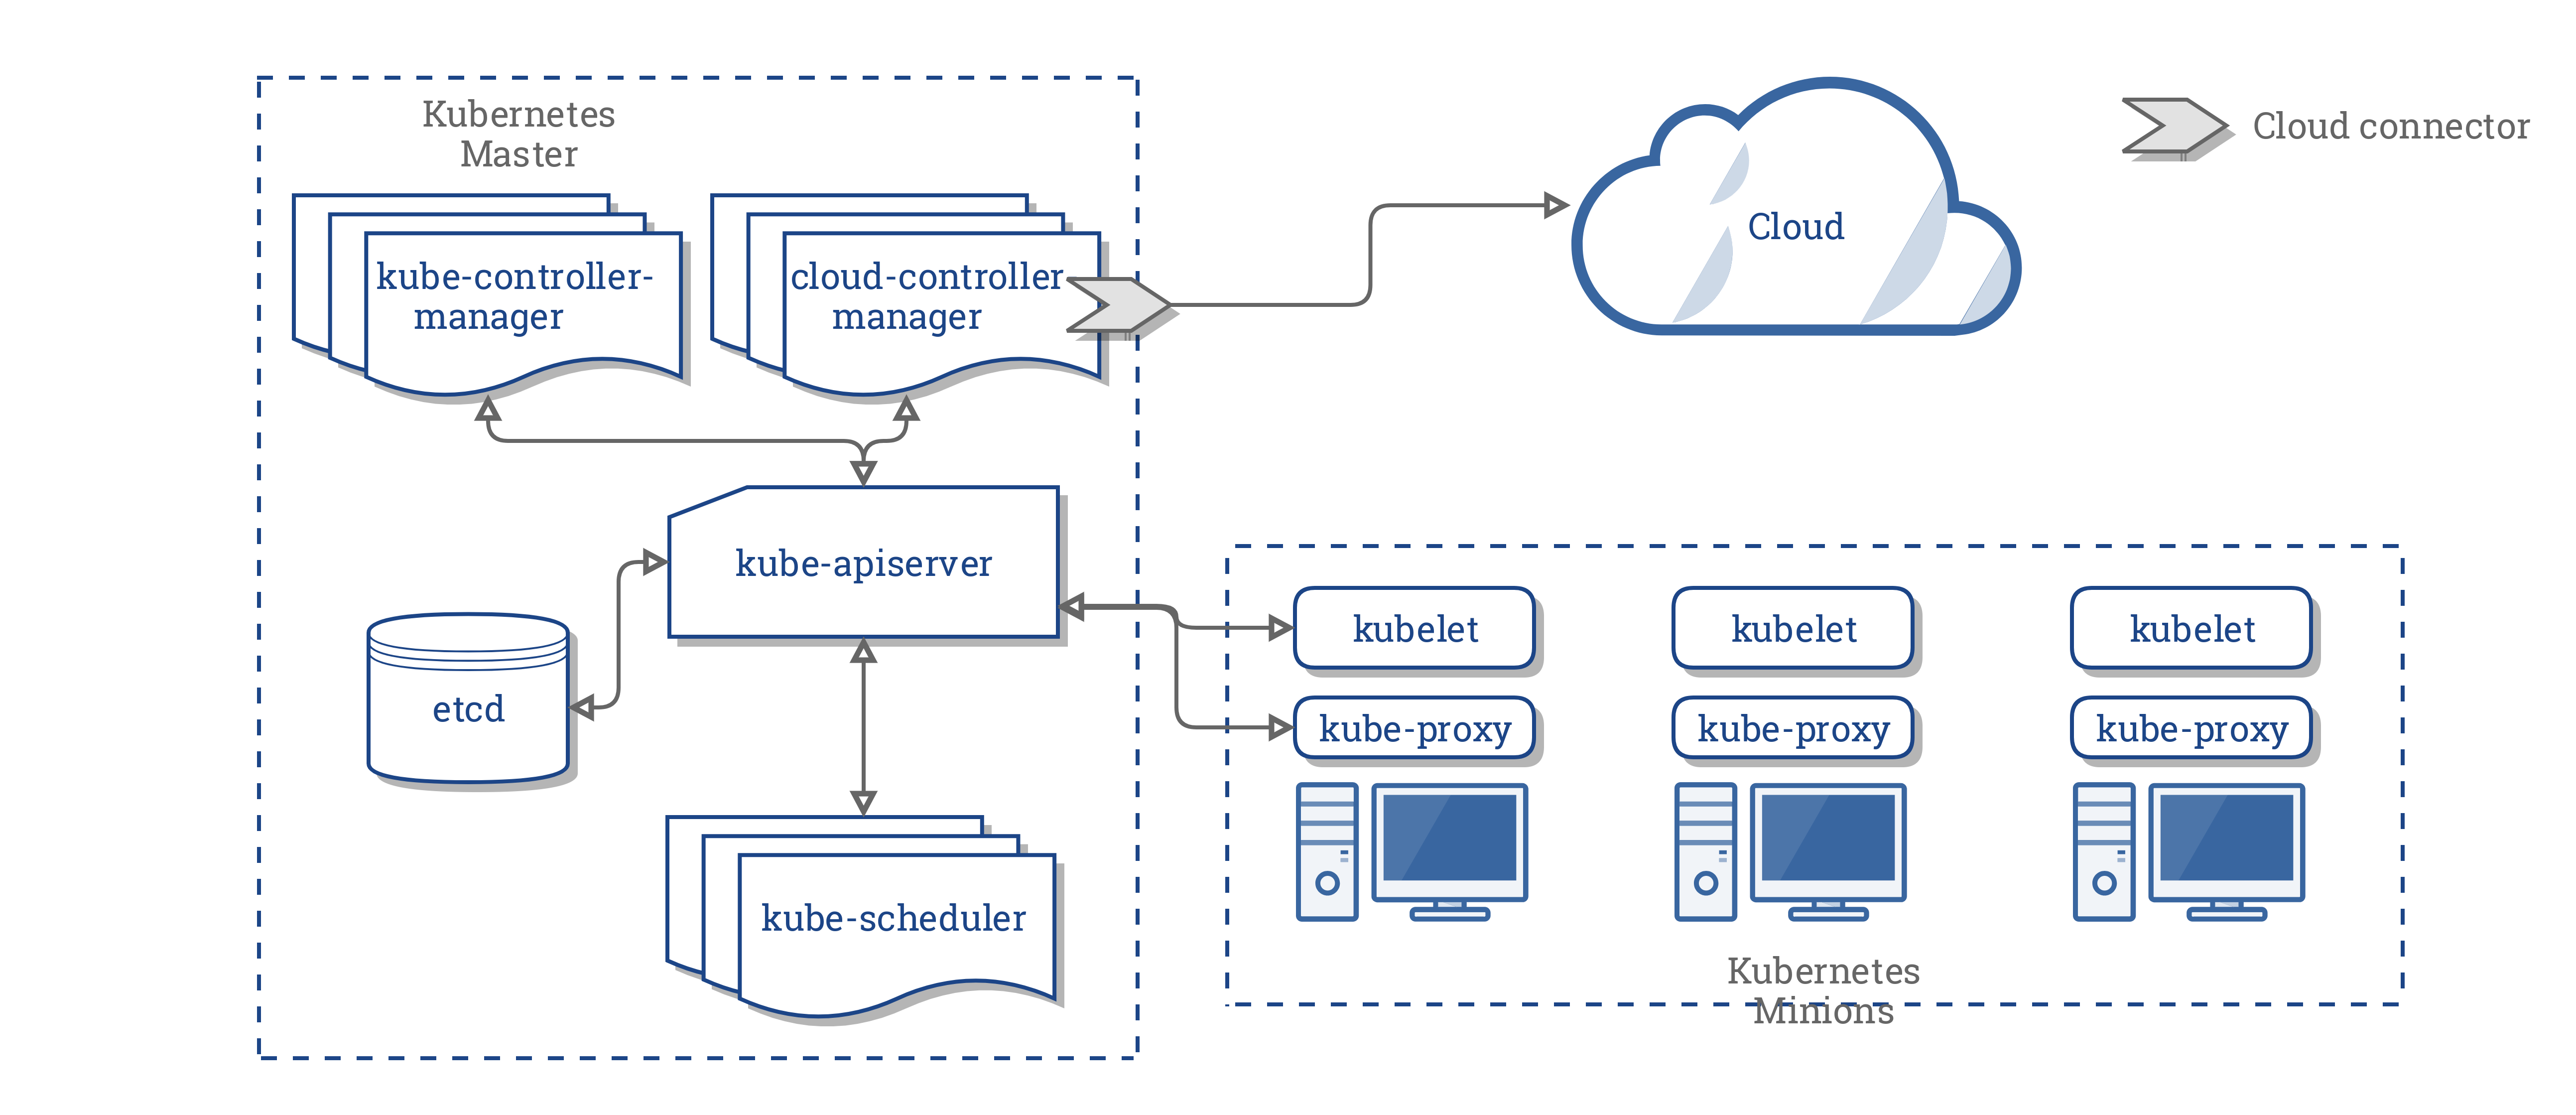
\includegraphics[width=1\columnwidth]{images/k8s-arch}
    \caption{Kubernetes architecture diagram\cite{k8s_arch}}
    \label{fig:k8s-arch}
\end{figure}

The Kubernetes nodes, also called workers or minions, run the actual workloads which are Linux containers using the Docker Engine. The kubelet component manages the state of the node which will accept resource offerings from the scheduler. The kube-proxy is responsible for managing the network on the node. It routes incoming traffic to the pod addresses and it can expose pods bundled as a service to the cluster, serving as a load balancer to the pods or services. 

\subsection{DC/OS}
\label{subsec:dcos}
\Gls{dcos} describes itself in the documentation\cite{dcos_what}: 
\begin{displayquote}
``As a datacenter operating system, DC/OS is itself a distributed system, a cluster manager, a container platform, and an operating system.''
\end{displayquote} 
Unlike a traditional operating system \gls{dcos} runs as a distributed operating system on different nodes and each node has its own host operating system. The master nodes accept tasks and schedule them on the agent nodes. Apache Mesos\cite{apache_mesos}, a distributed systems kernel, is responsible for the lifecycle of tasks. It launches schedulers on the slaves based on the type of tasks. Figure~\ref{fig:dcos-arch} shows an overview of all the components in a \gls{dcos} cluster. \Gls{dcos} has two built-in schedulers for scheduling Linux containers and two different container runtimes which can be seen in the container orchestration box on the master nodes in Figure~\ref{fig:dcos-arch}. 

\begin{figure}
    \centering
    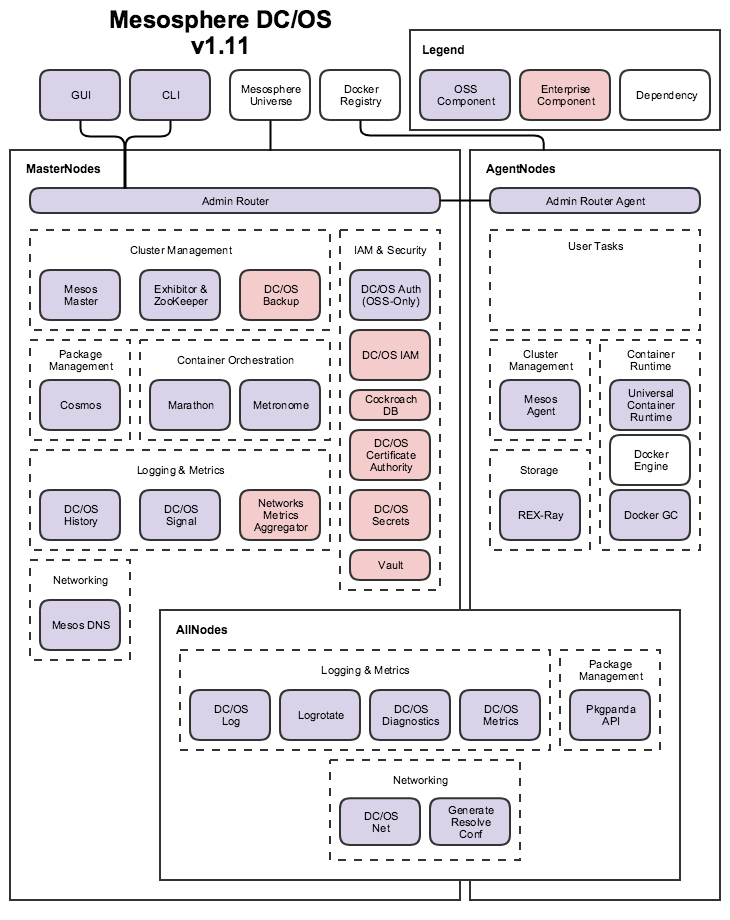
\includegraphics[width=1\columnwidth]{images/dcos-arch}
    \caption{\gls{dcos} architecture diagram\cite{dcos_arch}}
    \label{fig:dcos-arch}
\end{figure}

Marathon\cite{marathon} runs the actual container orchestration engine, allowing to schedule tasks and frameworks. A task could be an application inside a Docker image and a framework could be Kafka\cite{kafka} or Cassandra\cite{cassandra} which manage their own life cycle using Mesos. These frameworks and other services can be installed as a package from the Mesosphere Universe\cite{universe}. To periodically schedule jobs, operators can use Metronome\cite{metronome}, which allows to run jobs once or based on a regular schedule. On \gls{dcos} operators are not only limited to running containers, as binary executable can be launched and containerised at runtime. The Docker Engine is present on every slave to run the Docker images or operators can choose to use the Mesos \gls{ucr}\cite{ucr} to run Docker images and binary executables.

The technologies and components mentioned above make it possible to run different kind of workloads, not just containerised workloads. We can even run Kubernetes as a framework on \gls{dcos}, this way the Kubernetes scheduler will ask Mesos for resource offerings.

\section{CNI}
\label{sec:cni}
To deal with networking and containers the \gls{cni} specification was created, describing how to interact with network interfaces in Linux containers. This allows providers to write plugins to configure \gls{sdn} with container workloads. Mesos, \gls{dcos}, Kubernetes and even \gls{aws} have support for \gls{cni} plugins. Allowing operators to create virtual networks on container orchestration platforms.
The \gls{cni} specification only deals with creating and deleting network resources, it does not do network policies for example. Network policies need to be managed by the plugin itself, as every plugin has a different goal and ways of enforcing policies. A similar project exists for the Docker daemon called \gls{cnm}\cite{cnm, dua2016learning} implemented as libnetwork where developers can also develop new plugins. For example Project Calico provides plugins for both \gls{cni} and \gls{cnm} and both are installed when using the universe package from \gls{dcos}.

There is a set of standard provided plugins\cite{cni_plugin} that allow for basic operations like creating network interfaces and \gls{ipam}. Different kinds of interfaces can be created such as bridges, loopback interfaces and \glspl{vlan}. IP addresses can be either requested from a \gls{dhcp} server or maintained by a local database of allocated IPs. Other plugin providers can provide their own implementations of assigning IP address to containers.

\subsection{Project Calico}
\label{subsec:calico}
Project Calico uses a pure Layer 3 approach to enable virtual networking between container workloads. As opposed to traditional solutions which in most cases use overlay networks. Overlay networks have the extra burden of en- and decapsulating packages between workloads when the traffic crosses different machines. Without this Calico is able to save CPU cycles and makes it easier to understand packets on the wire. Performance tests\cite{dzone, dataplane, chunqi} show that Calico is able to achieve nearly identical throughput to directly connected workloads. Overlay networks, and other plugins such as Weave\cite{weave} are not able to reach this throughput.

Instead of using a vSwitch, Calico uses a vRouter to route traffic between containers. This vRouter uses the Layer 3 forwarding technique found in the Linux kernel. A local agent, called Felix, programs the routes from the containers to the host in the node's route table. Furthermore, a \gls{bird} is running on every node to advertise routes to containers on other nodes in the cluster. Figure~\ref{fig:hops} shows the hops made between two different containers or workloads. State information is exchanged using \gls{bgp} or route reflectors.

By default all containers can talk to each other in a Calico network. Operators want to separate traffic between different tenants of the compute cluster, by assigning policies. A policy is translated to a rule in iptables\cite{iptables} on the host, leveraging the default Linux firewall. This can even be extended to specific rules for different workloads within a tenancy. The policies are shared using a distributed key-value store called etcd\cite{etcd}, as can be seen in Figure~\ref{fig:calico-arch}.

\begin{figure}
    \centering
    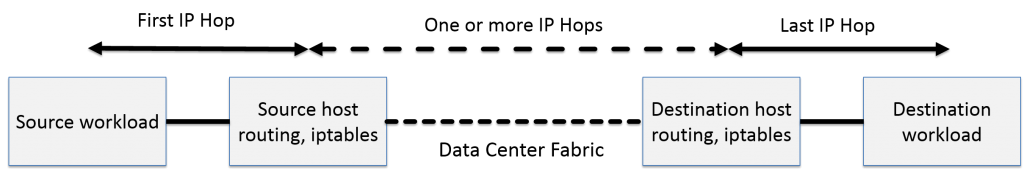
\includegraphics[width=1\columnwidth]{images/calico-hops}
    \caption{IP connectivity in Calico\cite{calico_learn}}
    \label{fig:hops}
\end{figure}

\subsection{Cilium}
\label{subsec:cilium}
A plugin that also takes a whole different approach is Cilium\cite{cilium} which allows for \gls{api} aware security policies. Instead of only operating at the network level with host and port based firewall rules, Cilium allows filtering of different protocols like \gls{http}, \gls{grpc}\cite{grpc} and Kafka\cite{kafka}. They do this by leveraging a new Linux kernel technology called \gls{bpf}\cite{mccanne1993bsd, cilium_bpf} by dynamically inserting \gls{bpf} bytecode into the Linux kernel, as can be seen in Figure~\ref{fig:cilium-arch}. 

This \gls{cni} plugin creates \gls{bpf} programs in the Linux kernel that control the network access. The \gls{bpf} programs are \gls{jit} compiled to CPU instructions to allow for native execution performance. Operators can do a lot of different things with this technology: simply monitoring the packets, redirecting packets and blocking packets. Only recent versions of the Linux kernel have \gls{bpf} capabilities, version 4.8.0 or newer is required. 

\begin{figure}
    \centering
    \begin{subfigure}[b]{0.49\textwidth}
    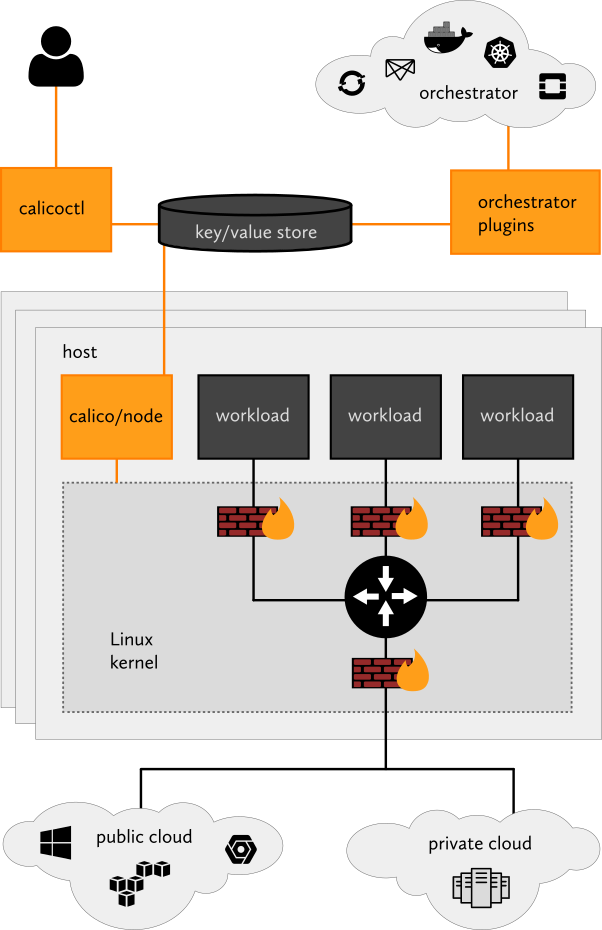
\includegraphics[width=0.8\textwidth]{images/calico-arch}
    \caption{Project Calico component overview\cite{calico_about}}
    \label{fig:calico-arch}
    \end{subfigure}
    \begin{subfigure}[b]{0.49\textwidth}
    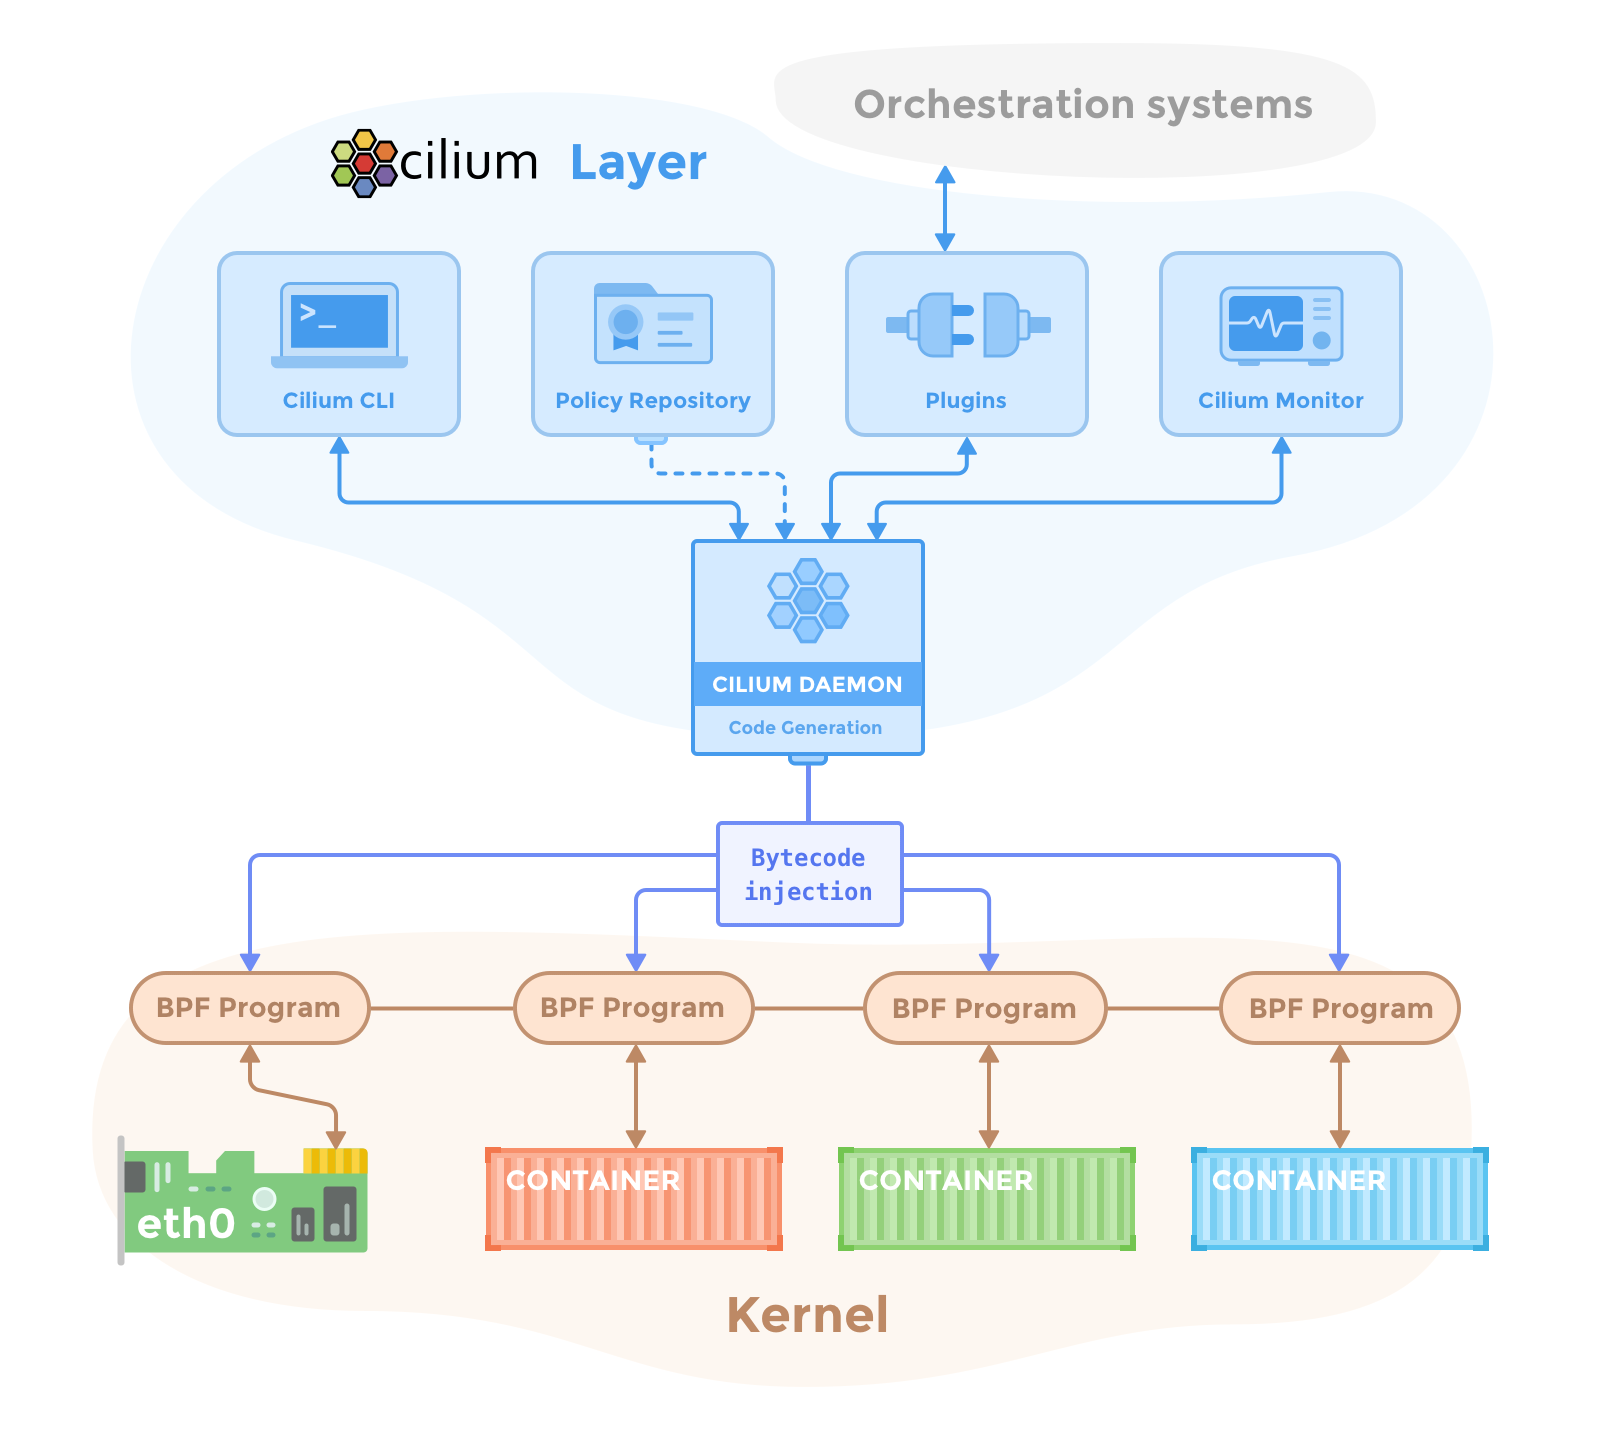
\includegraphics[width=\textwidth]{images/cilium-arch}
    \caption{Cilium component overview\cite{cilium_concepts}}
    \label{fig:cilium-arch}
    \end{subfigure}
\end{figure}
